\documentclass[11pt]{beamer}
\usetheme{Warsaw}
\usepackage[utf8]{inputenc}
\usepackage[spanish]{babel}
\usepackage{amsmath,amsthm,amssymb} %modos matemáticos y  simbolos
\usepackage{latexsym,amsfonts} %simbolos matematicos
\usepackage{graphicx}
\usepackage{physics} %Simbolos fisicos
\usepackage{array} %mejores formatos de tabla
\usepackage{tabulary}
\usepackage{multirow} %ocupar varias filas en una tabla
\usepackage{fancybox} %recuadros talegas
\usepackage{float} %ubicar graficas
\usepackage{color}
\usepackage{comment}
\usepackage{stackrel}
\usepackage{calligra}
\usepackage{lipsum} % texto de relleno
\usepackage{cite}
\author{Diego Sarceño}
\title{Multipletes y Números Leptónicos}
%\setbeamercovered{transparent} 
%\setbeamertemplate{navigation symbols}{} 
%\logo{} 
\institute{\footnotesize{201900109} \\ Escuela de Ciencias Físicas y Matemáticas} 
\date{\today} 
\subject{Capítulo $3.1.1.$} 
\begin{document}

\begin{frame}
\titlepage
\end{frame}

%\begin{frame}
%\tableofcontents
%\end{frame}

\frame{
	\frametitle{Generaciones}
	Existen $6$ Leptones, llamados generaciones, estos se conocen en pares
	$$ \mqty( \nu _e \\ e^- ), \qquad \qquad \mqty( \nu _\mu \\ \mu ^- ), \qquad \qquad \mqty( \nu _\tau \\ \tau ^- ). $$
	
	Donde, dada la gran masa, el $\mu ^-$ y $\tau ^-$ son los inestables.
}

\frame{
	\frametitle{Decaimiento del $\mu$}
	El muón decae por medio de procesos débiles en la siguiente forma
		$$ \mu ^+ \to e^+ + \nu _e + \bar{\nu} _\mu ; \qquad \qquad \mu ^- \to e^- + \bar{\nu} _e + \nu _\mu . $$
	Con un tiempo de vida de $(2.197019 \pm 0.000021) \times 10^{-6} s$.
}

\frame{
	\frametitle{Decaimiento del $\tau$}
	Esta es una partícula parecida el muón, pero dada su gran masa, tiene decaimientos a muchos estados finales como leptones y hadrones. Un $35\%$ de sus decaimientos son puramente leptónicos.
	Como por ejemplo
		$$ \tau ^+ \to \mu ^+ + \nu _\mu + \bar{\nu}_\tau ; \qquad \tau ^- \to e^- + \bar{\nu}_e + \nu _\tau . $$
	Con un tiempo de vida de $ (2.906 \pm 0.011)\times 10^{-13} s $.
}

\frame{
	\frametitle{Números Leptónicos}
	$$ L_e ,L_\mu ,L_\tau  $$
	Su valor es $1$ para su respectiva partícula y sabor de neutrino, $-1$ para antipartícula y $0$ para cualquier otra partícula que no sea leptón. (Esto obviamente para $1$ partícula)´
}

\frame{
	\frametitle{Números Leptónicos}
	\textbf{Ejemplo: }
	$$
	\left.\begin{array}{cccccccc}
		n & \to & p & + & e^- & + & \bar{\nu}_e &  \\
		\downarrow &  & \downarrow &  & \downarrow &  & \downarrow &  \\
		0 &  & 0 &  & +1 &  & -1 & = 0
	\end{array}\right.	
	$$
	Los decaimientos antes mostrados, ilustran una conservación en el número leptónico.
}

\frame{
	\frametitle{Números Leptónicos}
	Para interacciones electromagnéticas, lo anterior se reduce a $N(e^- ,\mu ^- ,\tau ^-) - N(e^+ ,\mu ^+ ,\tau ^+)$, interaccion en pares partícula-antipartícula. Por ejemplo
	\begin{figure}[H]
		\centering
		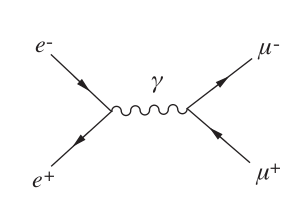
\includegraphics[scale=0.5]{img/em.png}
		\caption{Interacción: $ e^+ + e^- \to \mu ^+ + \mu ^- $}
	\end{figure}
}

\frame{
	\frametitle{Conservación del Número Leptónico}
	Así como en la conservación de la carga, las interacciones que no conserven el número leptónico no se dan en la naturaleza.
}

\frame{
	\frametitle{Ejemplo: } 
	$$ \nu _\mu + n \to e^- + p $$
	La cual viola $L_e$ y $L_\mu$, por lo que no es observada.
}

\frame{
	\frametitle{Estabilidad del Electrón}
	Todo lo anterior explica la estabilidad del electrón, es ligero y conserva la carga en todas las interacciones.
}

\frame{
	\frametitle{Tabla}
	\begin{figure}[H]
		\centering
		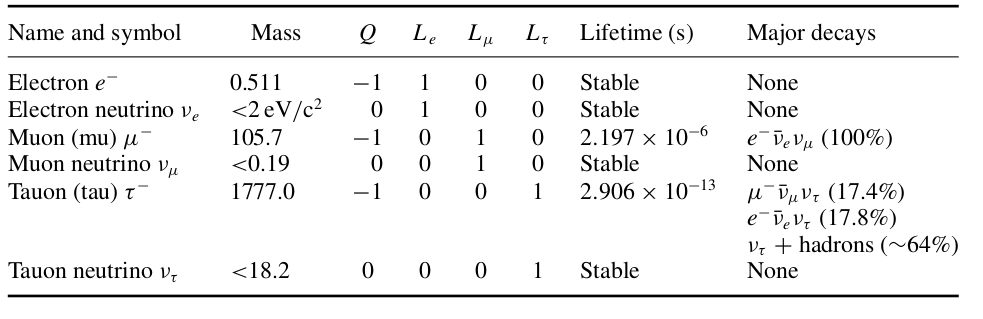
\includegraphics[scale=0.3]{img/table.png}
		\caption{Tabla de datos de leptónes.}
		\label{tabla}
	\end{figure}
}


\frame{
	\centering
	\vspace{1cm}
	GRACIAS POR SU ATENCIÓN
}

\frame{
	\frametitle{LINK}
	\url{https://youtu.be/yMd485WI_BY}
}














\end{document}